\section{Appendix}

\subsection{Number of modes and intractibility}\label{sec:modes}

Suppose that the pair $(\rho_{0},\rho_{1})$ is in the region \textbf{W}, then the list of possible combinations in Table \ref{table:modes} shows that $(\rho_{1},\rho_{2})$ can be either in \textbf{W} or \textbf{L}. Similarly, if $(\rho_{0},\rho_{1})$ is in the region \textbf{L}, $(\rho_{1},\rho_{2})$ can be either in \textbf{W} or \textbf{L}, and for $(\rho_{0},\rho_{1})$ in \textbf{D}, $(\rho_{1},\rho_{2})$ can be either in \textbf{W}, \textbf{L}, or \textbf{D}. As an example, figure \ref{fig:threeLevelModes} describes all the possible sixteen combinations for the first three pairs $(\rho_{0},\rho_{1})$, $(\rho_{1},\rho_{2})$, and $(\rho_{2},\rho_{3})$.

\begin{figure}[ht]
  \centering
    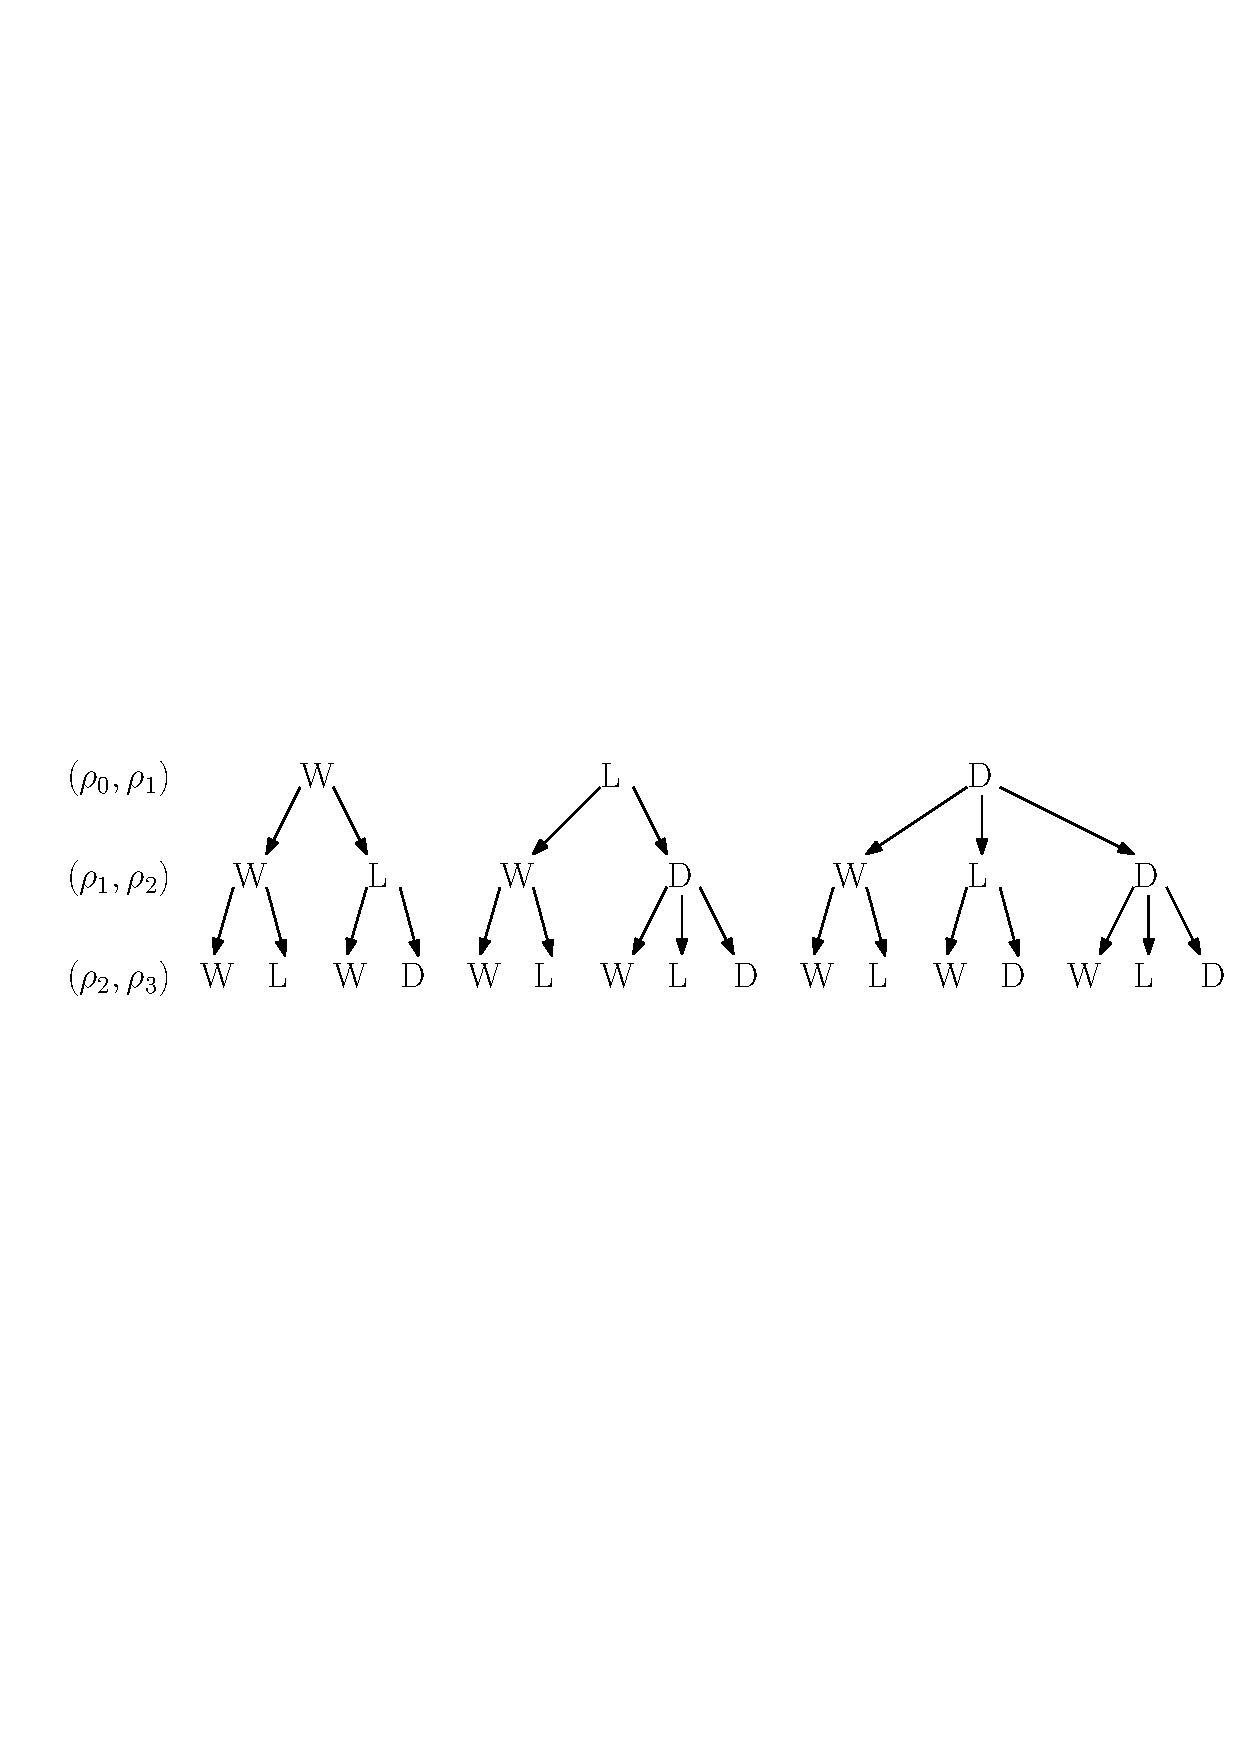
\includegraphics[width=8cm]{figures/threeLevelModes.pdf}
    \caption{The sixteen possible modes for the first three pairs $(\rho_{0},\rho_{1})$, $(\rho_{1},\rho_{2})$, and $(\rho_{2},\rho_{3})$.}
    \label{fig:threeLevelModes}
\end{figure}

We can recursively compute the number of ''modes'' $M_{k}$ with respect to $k$, where $k$ is the number of cells of the discretized link. Let's denote by $w_{k}$, $l_{k}$, and $d_{k}$ the number of modes for which $(\rho_{k},\rho_{k+1})$ is in \textbf{W}, \textbf{L}, and \textbf{D} respectively. Then we have these equations: 

\begin{equation}
w_{0} = l_{0} = d_{0} = 1
\label{eq:modes1}
\end{equation}

\begin{equation}
\begin{array}{lllllll}
w_{k+1} & = & w_{k} & + & l_{k} & + & d_{k}\\
l_{k+1} & = & w_{k} & + & d_{k} & & \\
d_{k+1} & = & l_{k} & + & d_{k} & &
\end{array} \quad \text{for }k \geq 0
\label{eq:modes2}
\end{equation}

\begin{equation}
n_{k} = w_{k} + l_{k} + d_{k} \quad \text{for }k \geq 0
\label{eq:modes3}
\end{equation}

Using matrix notations, equation (\ref{eq:modes2}) reads:

\begin{equation}
\left[ \begin{array}{c}
w_{k+1} \\
l_{k+1} \\
d_{k+1} \end{array} \right] = A \times 
\left[ \begin{array}{c}
w_{k} \\
l_{k} \\
d_{k} \end{array} \right]
\label{eq:modes4}
\end{equation}

\noindent where

\begin{equation}
A = \left[ \begin{array}{ccc}
1 & 1 & 1 \\
1 & 0 & 1 \\
0 & 1 & 1 \end{array} \right]
\label{eq:modes5}
\end{equation}

Then 

\begin{equation}
\left[ \begin{array}{c}
w_{k} \\
l_{k} \\
d_{k} \end{array} \right] = A^{k} \times 
\left[ \begin{array}{c}
w_{0} \\
l_{0} \\
d_{0} \end{array} \right]
\label{eq:modes6}
\end{equation}

It is possible to compute $A^{k}$ explicitly by diagonalizing the matrix $A$, to obtain an explicit expression for $w_{k}$, $l_{k}$, and $d_{k}$ in the form of $a.\beta^{k} + b.\gamma^{k} + c.\delta^{k}$. However, this analytical expression is unwieldy, so we will just derive lower and upper bounds to $n_{k}$. It is easy to see that $d_{k} \leq n_{k}/2$ for $k\geq 0$, then we can prove recursively that $3\cdot2^{k} \leq n_{k} \leq 3\cdot(2.5)^{k}$.

\begin{table}[ht]
\centering % used for centering table
\begin{tabular}{|c|c|c|c|c|c|}
  \hline
 number of cells & 1 & 2 & 5 & 10 & 20\\
  \hline
 number of modes & 7 & 16 & 182 & 10426 & 34206521\\
  \hline
 bound without analysis & 7 & 49 & 16807 & 282475249 & $8\cdot 10^{16}$\\
  \hline
\end{tabular}
\label{table:numModes} % is used to refer this table in the text
\caption{Number of modes for a homogeneous road.}
\end{table}

Even if we have found the minimal polyhedral partition of the space, the number of modes grows exponentially as the number of cells increases, so it is difficult to store all the possible modes. However, at any time step, the mode of each cell can be determined among the 7 possible modes and constructed sequentially building up the general mode of the segment of road.

\subsection{The heterogeneous case}\label{sec:CDFD}

\begin{figure}[ht]
  \centering
    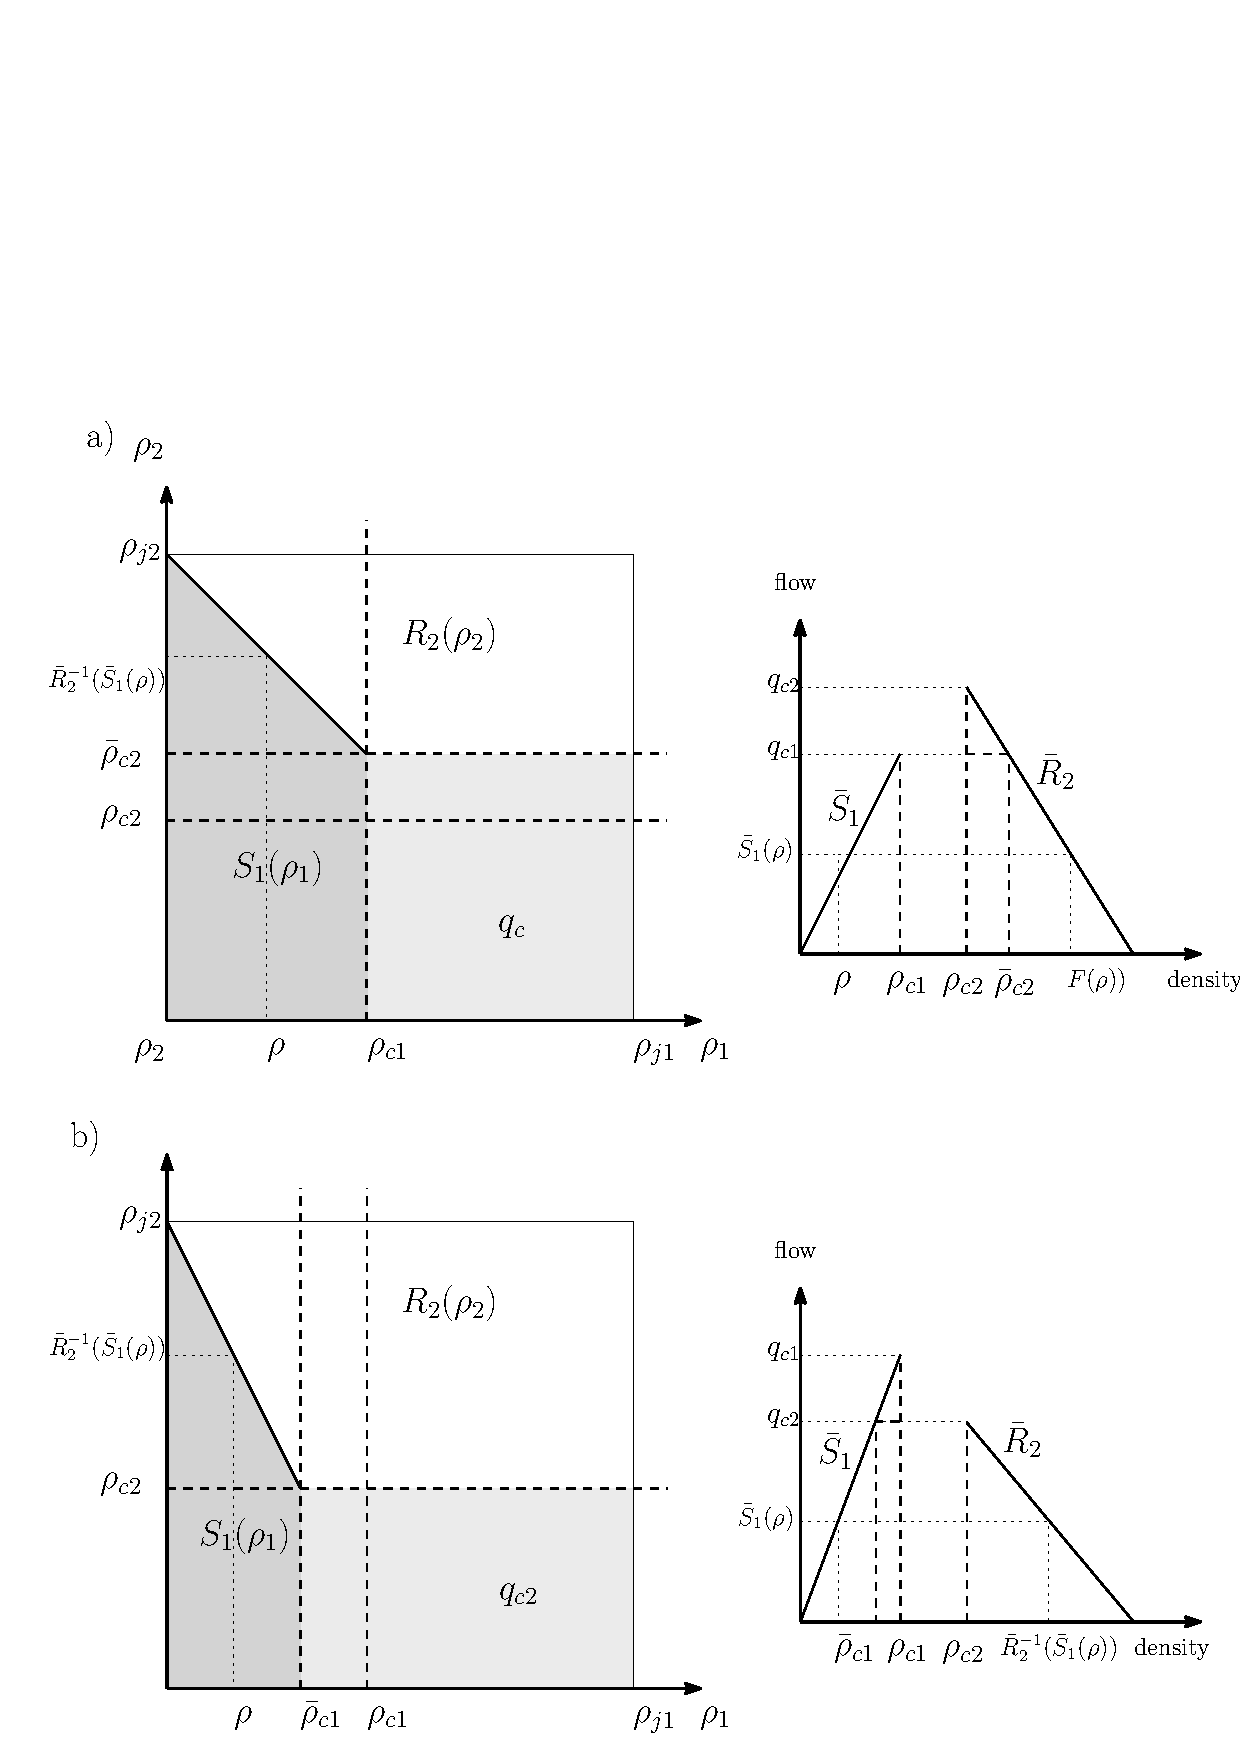
\includegraphics[width=8cm]{figures/godunovDiagram3.pdf}
    \caption{Values of $G(\rho_{1},\rho_{2})$ in the space $(\rho_{1},\rho_{2})$ for the Daganzo-Newell fundamental diagram with different capacities $q_{c1} < q_{c2}$ for a) and $q_{c1} > q_{c2}$ for b). Note that for illustration purposes we suppose $\rho_{c1}\leq\rho_{c2}$.}
    \label{fig:godunovDiagram3}
\end{figure}

In this section, we study the CTM for a heterogeneous road, i.e. $\omega_{f}$, $v_{f}$, $\rho_{j}$, $\rho_{c}$, $q_{c}$ can vary along the link and we add the subscript $i$: $\alpha_{i}$, $\omega_{fi}$, $v_{fi}$, $\rho_{ji}$, $\rho_{ci}$, $q_{ci}$ for the parameters of the fundamental diagram $Q_{i}$ at cell $i$, and the associated sending and receiving flows $S_{i}$, $R_{i}$. Figure \ref{fig:godunovDiagram3} shows the explicit values taken by $G(\rho_{1},\rho_{2})$ in different regions of the space $(\rho_{1},\rho_{2})$ when $q_{c1} < q_{c2}$. We note that the critical density $\rho_{c2}$ is increased to the \textit{effective} critical value $\bar{\rho}_{c2}$ for the receiving flow $R_{2}$, with $\bar{\rho}_{c2} = \bar{R}^{-1}_{2}(q_{c1})$, and the \textit{effective} capacity is $\bar{q}_{c} = q_{c1}$, which is the capacity of the sending flow $S_{1}$. And Figure \ref{fig:godunovDiagram3} also shows the explicit values taken by $G(\rho_{1},\rho_{2})$ in different regions of the space $(\rho_{1},\rho_{2})$ when $q_{c1} > q_{c2}$. Similarly, the critical density $\rho_{c1}$ is decreased to the \textit{effective} value $\bar{\rho}_{c1}$ for the sending flow $S_{1}$ with $\bar{\rho}_{c1} = \bar{S}^{-1}_{1}(q_{c2})$, and the \textit{effective} capacity is $\bar{q}_{c} = q_{c2}$, which is the capacity of the receiving flow $R_{2}$. The Godunov flux has a more general expression \ref{eq:rhoGodunovFlux2}:

\begin{equation}
G(\rho_{1},\rho_{2}) = \begin{cases}
R_{2}(\rho_{2}) & \text{if } (\rho_{1},\rho_{2}) \in \textbf{W}\\
\bar{q}_{c} & \text{if } (\rho_{1},\rho_{2}) \in \textbf{L}\\
S_{1}(\rho_{1}) & \text{if } (\rho_{1},\rho_{2}) \in \textbf{D}
\end{cases}
\label{eq:rhoGodunovFlux2}
\end{equation}

\begin{equation}
\begin{array}{lll}
\textbf{W} & = \{(\rho_{1},\rho_{2}) \mid & \rho_{2} > F(\rho_{1}) \text{ ,   } \rho_{2} > \bar{\rho}_{c2}\}\\
\textbf{L} & = \{(\rho_{1},\rho_{2}) \mid & \rho_{1} > \bar{\rho}_{c1} \text{ ,   } \rho_{2} \leq \bar{\rho}_{c2}\}\\
\textbf{D} & = \{(\rho_{1},\rho_{2}) \mid & \rho_{2} \leq F(\rho_{1}) \text{ ,   } \rho_{1} \leq \bar{\rho}_{c1}\}
\end{array}
\label{eq:regionsHetero}
\end{equation}

\noindent where the boundary between the white and grey regions follows the $(\rho_{1},\rho_{2})=(\rho_{1},F(\rho_{1}))$ trajectory with $F(\rho_{1})= \bar{R}^{-1}_{2}(\bar{S}_{1}(\rho_{1}))$ for $\rho_{1} \leq \rho_{c1}$. $\bar{S}$ and $\bar{R}$ denote the restrictions of the sending and receiving flows to the sub-regions $[0,\rho_{c})$ and $(\rho_{c},\rho_{j}]$ respectively, which also correspond to the left and right parts (w.r.t. $\rho_{c}$) of the fundamental diagram, as shown in the Figure \ref{fig:godunovDiagram3}.

\noindent When the velocity is the Daganzo-Newell function (\ref{eq:dnVelocity}), the Godunov Flux \ref{eq:rhoGodunovFlux2} becomes \ref{eq:rhoGodunovFlux3}:

\begin{equation} \label{eq:rhoGodunovFlux3a}
G_{DN}(\rho_{1},\rho_{2}) = \begin{cases}
-\omega_{f2} \left( \rho_{2} - \rho_{j2} \right) & \text{if } (\rho_{1},\rho_{2}) \in \textbf{W}\\
\bar{q}_{c} & \text{if } (\rho_{1},\rho_{2}) \in \textbf{L}\\
v_{f1} \rho_{1} & \text{if } (\rho_{1},\rho_{2}) \in \textbf{D}
\end{cases}
\end{equation}

\noindent and the boundary between the white and dark-grey regions is:

\begin{equation} \label{eq:boundaryHetero}
(\rho_{1},\rho_{2})=(\rho_{1},-\frac{v_{f1}}{\omega_{f2}}\rho_{1}+\rho_{j2})
\end{equation}

\noindent And \textbf{W}, \textbf{L}, \textbf{D} form a polyhedral partition of the space:

\begin{equation}
\begin{array}{lll}
\textbf{W} & = \{(\rho_{1},\rho_{2}) \mid & \rho_{2} + \frac{v_{f1}}{\omega_{f2}}\rho_{1} > \rho_{j2} \text{ ,   } \rho_{2} > \bar{\rho}_{c2}\}\\
\textbf{L} & = \{(\rho_{1},\rho_{2}) \mid & \rho_{1} > \bar{\rho}_{c1} \text{ ,   } \rho_{2} \leq \bar{\rho}_{c2}\}\\
\textbf{D} & = \{(\rho_{1},\rho_{2}) \mid & \rho_{2} + \frac{v_{f1}}{\omega_{f2}}\rho_{1} \leq \rho_{j2} \text{ ,   } \rho_{1} \leq \bar{\rho}_{c1}\}
\end{array}
\label{eq:regions4}
\end{equation}

At cell $i$, this implies the effective density $\bar{\rho}^{u}_{ci}$ associated with the upstream boundary can be different from the effective density $\bar{\rho}^{d}_{ci}$ associated with the downstream boundary, depending of the capacity drops at these boundaries. Hence, using the notations introduced in section \ref{sec:decompositionModes} all the combinations between $(\rho_{-},\rho)$ and $(\rho,\rho_{+})$ can be possible so we have nine modes. Consequently, for a discretization in $n$ cells, the number of possible modes is $3^{n+1}$.

\begin{table}[ht]
\centering % used for centering table
\begin{tabular}{|c|c|c|c|c|c|}
  \hline
 number of cells & 1 & 2 & 5 & 10 & 20\\
  \hline
 number of modes & 9 & 27 & 729 & 177147 & $10^{10}$\\
  \hline
\end{tabular}
\label{table:numModes2} % is used to refer this table in the text
\caption{Number of modes for a heterogeneous road.}
\end{table}
